%#########################1########################

 \cajita{%
Evolución del salario mínimo }%
{%
El salario mínimo diario se ubicó en el 2015 en Q 78.7 para las actividades agrícolas y las no agrícolas, el cual comparado con el 2011, tuvo un incremento del 23.6\%. 

Para las actividades de exportación y de maquila fue de 72.4 quetzales, cuyo incremento respecto del 2011 fue del 21.7\%. 

}%
{%
 Salario mínimo diario según rama de actividad económica} %
{%
 República de Guatemala, serie histórica, en quetzales corrientes} %
{%
 \begin{tikzpicture}[x=1pt,y=1pt]  % Created by tikzDevice version 0.9 on 2016-03-03 04:33:50
% !TEX encoding = UTF-8 Unicode
\definecolor{fillColor}{RGB}{255,255,255}
\path[use as bounding box,fill=fillColor,fill opacity=0.00] (0,0) rectangle (289.08,198.74);
\begin{scope}
\path[clip] (  0.00,  0.00) rectangle (289.08,198.74);

\path[] (  0.00,  0.00) rectangle (289.08,198.74);
\end{scope}
\begin{scope}
\path[clip] (  0.00,  0.00) rectangle (289.08,198.74);

\path[] (  0.00, 18.46) rectangle (289.08,164.23);

\path[] ( 33.36, 18.46) --
	( 33.36,164.23);

\path[] ( 88.95, 18.46) --
	( 88.95,164.23);

\path[] (144.54, 18.46) --
	(144.54,164.23);

\path[] (200.13, 18.46) --
	(200.13,164.23);

\path[] (255.72, 18.46) --
	(255.72,164.23);
\definecolor{drawColor}{RGB}{0,0,255}
\definecolor{fillColor}{RGB}{0,0,255}

\path[draw=drawColor,line width= 0.6pt,line join=round,fill=fillColor] (  9.27, 18.46) rectangle ( 24.09,136.42);
\definecolor{drawColor}{RGB}{157,187,255}
\definecolor{fillColor}{RGB}{157,187,255}

\path[draw=drawColor,line width= 0.6pt,line join=round,fill=fillColor] ( 25.94, 18.46) rectangle ( 40.77,136.42);
\definecolor{drawColor}{RGB}{200,200,200}
\definecolor{fillColor}{RGB}{200,200,200}

\path[draw=drawColor,line width= 0.6pt,line join=round,fill=fillColor] ( 42.62, 18.46) rectangle ( 57.45,128.55);
\definecolor{drawColor}{RGB}{0,0,255}
\definecolor{fillColor}{RGB}{0,0,255}

\path[draw=drawColor,line width= 0.6pt,line join=round,fill=fillColor] ( 64.86, 18.46) rectangle ( 79.68,144.38);
\definecolor{drawColor}{RGB}{157,187,255}
\definecolor{fillColor}{RGB}{157,187,255}

\path[draw=drawColor,line width= 0.6pt,line join=round,fill=fillColor] ( 81.54, 18.46) rectangle ( 96.36,144.38);
\definecolor{drawColor}{RGB}{200,200,200}
\definecolor{fillColor}{RGB}{200,200,200}

\path[draw=drawColor,line width= 0.6pt,line join=round,fill=fillColor] ( 98.21, 18.46) rectangle (113.04,134.20);
\definecolor{drawColor}{RGB}{0,0,255}
\definecolor{fillColor}{RGB}{0,0,255}

\path[draw=drawColor,line width= 0.6pt,line join=round,fill=fillColor] (120.45, 18.46) rectangle (135.27,150.68);
\definecolor{drawColor}{RGB}{157,187,255}
\definecolor{fillColor}{RGB}{157,187,255}

\path[draw=drawColor,line width= 0.6pt,line join=round,fill=fillColor] (137.13, 18.46) rectangle (151.95,150.68);
\definecolor{drawColor}{RGB}{200,200,200}
\definecolor{fillColor}{RGB}{200,200,200}

\path[draw=drawColor,line width= 0.6pt,line join=round,fill=fillColor] (153.81, 18.46) rectangle (168.63,139.99);
\definecolor{drawColor}{RGB}{0,0,255}
\definecolor{fillColor}{RGB}{0,0,255}

\path[draw=drawColor,line width= 0.6pt,line join=round,fill=fillColor] (176.04, 18.46) rectangle (190.87,157.29);
\definecolor{drawColor}{RGB}{157,187,255}
\definecolor{fillColor}{RGB}{157,187,255}

\path[draw=drawColor,line width= 0.6pt,line join=round,fill=fillColor] (192.72, 18.46) rectangle (207.54,157.29);
\definecolor{drawColor}{RGB}{200,200,200}
\definecolor{fillColor}{RGB}{200,200,200}

\path[draw=drawColor,line width= 0.6pt,line join=round,fill=fillColor] (209.40, 18.46) rectangle (224.22,146.07);
\definecolor{drawColor}{RGB}{0,0,255}
\definecolor{fillColor}{RGB}{0,0,255}

\path[draw=drawColor,line width= 0.6pt,line join=round,fill=fillColor] (231.63, 18.46) rectangle (246.46,164.23);
\definecolor{drawColor}{RGB}{157,187,255}
\definecolor{fillColor}{RGB}{157,187,255}

\path[draw=drawColor,line width= 0.6pt,line join=round,fill=fillColor] (248.31, 18.46) rectangle (263.14,164.23);
\definecolor{drawColor}{RGB}{200,200,200}
\definecolor{fillColor}{RGB}{200,200,200}

\path[draw=drawColor,line width= 0.6pt,line join=round,fill=fillColor] (264.99, 18.46) rectangle (279.81,152.45);
\definecolor{drawColor}{RGB}{0,0,0}

\path[draw=drawColor,line width= 0.6pt,line join=round] (  0.00, 18.46) -- (289.08, 18.46);

\node[text=drawColor,rotate= 90.00,anchor=base west,inner sep=0pt, outer sep=0pt, scale=  0.83] at ( 19.91,138.97) {63.7};

\node[text=drawColor,rotate= 90.00,anchor=base west,inner sep=0pt, outer sep=0pt, scale=  0.83] at ( 36.59,138.97) {63.7};

\node[text=drawColor,rotate= 90.00,anchor=base west,inner sep=0pt, outer sep=0pt, scale=  0.83] at ( 53.27,131.10) {59.5};

\node[text=drawColor,rotate= 90.00,anchor=base west,inner sep=0pt, outer sep=0pt, scale=  0.83] at ( 75.50,146.93) {68.0};

\node[text=drawColor,rotate= 90.00,anchor=base west,inner sep=0pt, outer sep=0pt, scale=  0.83] at ( 92.18,146.93) {68.0};

\node[text=drawColor,rotate= 90.00,anchor=base west,inner sep=0pt, outer sep=0pt, scale=  0.83] at (108.86,136.74) {62.5};

\node[text=drawColor,rotate= 90.00,anchor=base west,inner sep=0pt, outer sep=0pt, scale=  0.83] at (131.10,153.23) {71.4};

\node[text=drawColor,rotate= 90.00,anchor=base west,inner sep=0pt, outer sep=0pt, scale=  0.83] at (147.77,153.23) {71.4};

\node[text=drawColor,rotate= 90.00,anchor=base west,inner sep=0pt, outer sep=0pt, scale=  0.83] at (164.45,142.54) {65.6};

\node[text=drawColor,rotate= 90.00,anchor=base west,inner sep=0pt, outer sep=0pt, scale=  0.83] at (186.69,159.84) {75.0};

\node[text=drawColor,rotate= 90.00,anchor=base west,inner sep=0pt, outer sep=0pt, scale=  0.83] at (203.37,159.84) {75.0};

\node[text=drawColor,rotate= 90.00,anchor=base west,inner sep=0pt, outer sep=0pt, scale=  0.83] at (220.04,148.61) {68.9};

\node[text=drawColor,rotate= 90.00,anchor=base west,inner sep=0pt, outer sep=0pt, scale=  0.83] at (242.28,166.78) {78.7};

\node[text=drawColor,rotate= 90.00,anchor=base west,inner sep=0pt, outer sep=0pt, scale=  0.83] at (258.96,166.78) {78.7};

\node[text=drawColor,rotate= 90.00,anchor=base west,inner sep=0pt, outer sep=0pt, scale=  0.83] at (275.64,155.00) {72.4};

\path[] (  0.00, 18.46) rectangle (289.08,164.23);
\end{scope}
\begin{scope}
\path[clip] (  0.00,  0.00) rectangle (289.08,198.74);

\path[] (  0.00, 18.46) --
	(289.08, 18.46);
\end{scope}
\begin{scope}
\path[clip] (  0.00,  0.00) rectangle (289.08,198.74);

\path[] ( 33.36, 15.71) --
	( 33.36, 18.46);

\path[] ( 88.95, 15.71) --
	( 88.95, 18.46);

\path[] (144.54, 15.71) --
	(144.54, 18.46);

\path[] (200.13, 15.71) --
	(200.13, 18.46);

\path[] (255.72, 15.71) --
	(255.72, 18.46);
\end{scope}
\begin{scope}
\path[clip] (  0.00,  0.00) rectangle (289.08,198.74);
\definecolor{drawColor}{RGB}{0,0,0}

\node[text=drawColor,anchor=base,inner sep=0pt, outer sep=0pt, scale=  1.00] at ( 33.36,  5.69) {2011};

\node[text=drawColor,anchor=base,inner sep=0pt, outer sep=0pt, scale=  1.00] at ( 88.95,  5.69) {2012};

\node[text=drawColor,anchor=base,inner sep=0pt, outer sep=0pt, scale=  1.00] at (144.54,  5.69) {2013};

\node[text=drawColor,anchor=base,inner sep=0pt, outer sep=0pt, scale=  1.00] at (200.13,  5.69) {2014};

\node[text=drawColor,anchor=base,inner sep=0pt, outer sep=0pt, scale=  1.00] at (255.72,  5.69) {2015};
\end{scope}
\begin{scope}
\path[clip] (  0.00,  0.00) rectangle (289.08,198.74);
\coordinate (apoyo1) at (31.76,188.79);
\coordinate (apoyo2) at (118.73,188.79);
\coordinate (apoyo3) at (215.96,188.79);
\coordinate (longitudFicticia) at (7.11,9.95);
\coordinate (longitud) at (7.11,7.11);
\coordinate (desY) at (0,1.42);
\definecolor[named]{ct1}{HTML}{
0000FF
}
\definecolor[named]{ct2}{HTML}{
9DBBFF
}
\definecolor[named]{ct3}{HTML}{
C8C8C8
}
\definecolor[named]{ctb1}{HTML}{
0000FF
}
\definecolor[named]{ctb2}{HTML}{
9DBBFF
}
\definecolor[named]{ctb3}{HTML}{
C8C8C8
}
\path [fill=none] (apoyo1) rectangle ($(apoyo1)+(longitudFicticia)$)
node [xshift=0.3cm,inner sep=0pt, outer sep=0pt,text width=1.33333333333333in,midway,right,scale = 0.9]{Agrícola};
\draw [color= ctb1, fill=ct1] ( $(apoyo1)  + (desY) $) rectangle ($(apoyo1)+ (desY) +(longitud)$);
\path [fill=none] (apoyo2) rectangle ($(apoyo2)+(longitudFicticia)$)
node [xshift=0.3cm,inner sep=0pt, outer sep=0pt,text width=1.33333333333333in,midway,right,scale = 0.9]{No agrícola};
\draw [color = ctb2, fill=ct2] ( $(apoyo2)  + (desY) $) rectangle ($(apoyo2)+ (desY) +(longitud)$);
\path [fill=none] (apoyo3) rectangle ($(apoyo3)+(longitudFicticia)$)
node [xshift=0.3cm,inner sep=0pt, outer sep=0pt,text width=1.33333333333333in,midway,right,scale = 0.9]{Maquila};
\path [color = ctb3, fill=ct3] ( $(apoyo3)  + (desY) $) rectangle ($(apoyo3)+ (desY) +(longitud)$);
\end{scope}
  \end{tikzpicture}}%
{%
 Instituto Nacional de Estadística} %


%#########################2########################

\cajita{%
	Ingreso laboral mensual }%
{%
De acuerdo a los datos de la Encuesta Nacional de Empleo e Ingresos, el salario laboral mensual promedio para el país en el 2014 fue de Q 2,207, el cual respecto del 2011 representó un incremento del 31.0\%. }%
{%
	Ingreso laboral mensual promedio} %
{%
	República de Guatemala, serie histórica por ENEI, en quetzales corrientes} %
{%
	\begin{tikzpicture}[x=1pt,y=1pt]  % Created by tikzDevice version 0.9 on 2016-03-03 04:33:56
% !TEX encoding = UTF-8 Unicode
\definecolor{fillColor}{RGB}{255,255,255}
\path[use as bounding box,fill=fillColor,fill opacity=0.00] (0,0) rectangle (289.08,198.74);
\begin{scope}
\path[clip] (  0.00,  0.00) rectangle (289.08,198.74);

\path[] (  0.00,  0.00) rectangle (289.08,198.74);
\end{scope}
\begin{scope}
\path[clip] (  0.00,  0.00) rectangle (289.08,198.74);

\path[] (  8.24, 15.61) rectangle (280.54,191.48);

\path[] (  8.24, 46.37) --
	(280.54, 46.37);

\path[] (  8.24,105.27) --
	(280.54,105.27);

\path[] (  8.24,164.17) --
	(280.54,164.17);

\path[] (  8.24, 16.92) --
	(280.54, 16.92);

\path[] (  8.24, 75.82) --
	(280.54, 75.82);

\path[] (  8.24,134.72) --
	(280.54,134.72);

\path[] ( 39.66, 15.61) --
	( 39.66,191.48);

\path[] ( 92.03, 15.61) --
	( 92.03,191.48);

\path[] (144.39, 15.61) --
	(144.39,191.48);

\path[] (196.76, 15.61) --
	(196.76,191.48);

\path[] (249.12, 15.61) --
	(249.12,191.48);
\definecolor{drawColor}{RGB}{0,0,255}

\path[draw=drawColor,line width= 1.7pt,line join=round] ( 39.66, 60.50) --
	( 92.03, 72.05) --
	(144.39,109.51) --
	(196.76,154.27) --
	(249.12,183.49);
\definecolor{drawColor}{RGB}{0,0,0}

\node[text=drawColor,anchor=base,inner sep=0pt, outer sep=0pt, scale=  1.02] at ( 39.66, 48.59) {1,685};

\node[text=drawColor,anchor=base east,inner sep=0pt, outer sep=0pt, scale=  1.02] at ( 88.01, 72.05) {1,734};

\node[text=drawColor,anchor=base east,inner sep=0pt, outer sep=0pt, scale=  1.02] at (140.37,109.51) {1,893};

\node[text=drawColor,anchor=base east,inner sep=0pt, outer sep=0pt, scale=  1.02] at (192.74,154.27) {2,083};

\node[text=drawColor,anchor=base,inner sep=0pt, outer sep=0pt, scale=  1.02] at (249.12,187.46) {2,207};

\path[draw=drawColor,line width= 0.1pt,line join=round] (  8.24, 23.61) -- (280.54, 23.61);

\path[] (  8.24, 15.61) rectangle (280.54,191.48);
\end{scope}
\begin{scope}
\path[clip] (  0.00,  0.00) rectangle (289.08,198.74);

\path[] (  8.24, 15.61) --
	(  8.24,191.48);
\end{scope}
\begin{scope}
\path[clip] (  0.00,  0.00) rectangle (289.08,198.74);
\definecolor{drawColor}{RGB}{255,255,255}

\node[text=drawColor,text opacity=0.00,anchor=base east,inner sep=0pt, outer sep=0pt, scale=  1.00] at (  3.29, 13.01) {1500};

\node[text=drawColor,text opacity=0.00,anchor=base east,inner sep=0pt, outer sep=0pt, scale=  1.00] at (  3.29, 71.91) {1750};

\node[text=drawColor,text opacity=0.00,anchor=base east,inner sep=0pt, outer sep=0pt, scale=  1.00] at (  3.29,130.81) {2000};
\end{scope}
\begin{scope}
\path[clip] (  0.00,  0.00) rectangle (289.08,198.74);

\path[] (  5.49, 16.92) --
	(  8.24, 16.92);

\path[] (  5.49, 75.82) --
	(  8.24, 75.82);

\path[] (  5.49,134.72) --
	(  8.24,134.72);
\end{scope}
\begin{scope}
\path[clip] (  0.00,  0.00) rectangle (289.08,198.74);

\path[] (  8.24, 15.61) --
	(280.54, 15.61);
\end{scope}
\begin{scope}
\path[clip] (  0.00,  0.00) rectangle (289.08,198.74);

\path[] ( 39.66, 12.86) --
	( 39.66, 15.61);

\path[] ( 92.03, 12.86) --
	( 92.03, 15.61);

\path[] (144.39, 12.86) --
	(144.39, 15.61);

\path[] (196.76, 12.86) --
	(196.76, 15.61);

\path[] (249.12, 12.86) --
	(249.12, 15.61);
\end{scope}
\begin{scope}
\path[clip] (  0.00,  0.00) rectangle (289.08,198.74);
\definecolor{drawColor}{RGB}{0,0,0}

\node[text=drawColor,anchor=base,inner sep=0pt, outer sep=0pt, scale=  1.00] at ( 39.66,  2.85) {2011};

\node[text=drawColor,anchor=base,inner sep=0pt, outer sep=0pt, scale=  1.00] at ( 92.03,  2.85) {2012};

\node[text=drawColor,anchor=base,inner sep=0pt, outer sep=0pt, scale=  1.00] at (144.39,  2.85) {2013};

\node[text=drawColor,anchor=base,inner sep=0pt, outer sep=0pt, scale=  1.00] at (196.76,  2.85) {2014};

\node[text=drawColor,anchor=base,inner sep=0pt, outer sep=0pt, scale=  1.00] at (249.12,  2.85) {2015};
\end{scope}
  \end{tikzpicture}}%
{%
	ENEI 2011, 2012, 2-2013, 1-2014.} %


%#########################3########################

\cajita{%
	Ingreso laboral mensual según dominio de estudio}%
{%
De acuerdo a los dominios de estudio de las ENEI, en el 2014 el salario promedio en urbano metropolitano fue mayor al resto urbano y al rural en un 9.7\%  y 99.3\%, respectivamente.

Respecto a la variación de los salarios, en relación al 2011, tuvieron un incremento del 10\% para el dominio urbano metropolitano, del 55\% para el resto urbano y del 20\% para el rural.}%
{%
	Promedio del ingreso laboral mensual según dominio de estudio} %
{%
	República de Guatemala, serie histórica de ENEI, en quetzales corrientes} %
{%
	\begin{tikzpicture}[x=1pt,y=1pt]  % Created by tikzDevice version 0.9 on 2016-03-03 04:34:05
% !TEX encoding = UTF-8 Unicode
\definecolor{fillColor}{RGB}{255,255,255}
\path[use as bounding box,fill=fillColor,fill opacity=0.00] (0,0) rectangle (289.08,198.74);
\begin{scope}
\path[clip] (  0.00,  0.00) rectangle (289.08,198.74);

\path[] (  0.00,  0.00) rectangle (289.08,198.74);
\end{scope}
\begin{scope}
\path[clip] (  0.00,  0.00) rectangle (289.08,198.74);

\path[] (  0.00, 18.46) rectangle (289.08,159.90);

\path[] ( 41.30, 18.46) --
	( 41.30,159.90);

\path[] (110.13, 18.46) --
	(110.13,159.90);

\path[] (178.95, 18.46) --
	(178.95,159.90);

\path[] (247.78, 18.46) --
	(247.78,159.90);
\definecolor{drawColor}{RGB}{0,0,255}
\definecolor{fillColor}{RGB}{0,0,255}

\path[draw=drawColor,line width= 0.6pt,line join=round,fill=fillColor] ( 11.47, 18.46) rectangle ( 29.83,146.72);
\definecolor{drawColor}{RGB}{157,187,255}
\definecolor{fillColor}{RGB}{157,187,255}

\path[draw=drawColor,line width= 0.6pt,line join=round,fill=fillColor] ( 32.12, 18.46) rectangle ( 50.47,101.44);
\definecolor{drawColor}{RGB}{200,200,200}
\definecolor{fillColor}{RGB}{200,200,200}

\path[draw=drawColor,line width= 0.6pt,line join=round,fill=fillColor] ( 52.77, 18.46) rectangle ( 71.12, 77.50);
\definecolor{drawColor}{RGB}{0,0,255}
\definecolor{fillColor}{RGB}{0,0,255}

\path[draw=drawColor,line width= 0.6pt,line join=round,fill=fillColor] ( 80.30, 18.46) rectangle ( 98.65,145.32);
\definecolor{drawColor}{RGB}{157,187,255}
\definecolor{fillColor}{RGB}{157,187,255}

\path[draw=drawColor,line width= 0.6pt,line join=round,fill=fillColor] (100.95, 18.46) rectangle (119.30,107.14);
\definecolor{drawColor}{RGB}{200,200,200}
\definecolor{fillColor}{RGB}{200,200,200}

\path[draw=drawColor,line width= 0.6pt,line join=round,fill=fillColor] (121.60, 18.46) rectangle (139.95, 79.19);
\definecolor{drawColor}{RGB}{0,0,255}
\definecolor{fillColor}{RGB}{0,0,255}

\path[draw=drawColor,line width= 0.6pt,line join=round,fill=fillColor] (149.13, 18.46) rectangle (167.48,149.47);
\definecolor{drawColor}{RGB}{157,187,255}
\definecolor{fillColor}{RGB}{157,187,255}

\path[draw=drawColor,line width= 0.6pt,line join=round,fill=fillColor] (169.78, 18.46) rectangle (188.13,110.52);
\definecolor{drawColor}{RGB}{200,200,200}
\definecolor{fillColor}{RGB}{200,200,200}

\path[draw=drawColor,line width= 0.6pt,line join=round,fill=fillColor] (190.43, 18.46) rectangle (208.78, 89.81);
\definecolor{drawColor}{RGB}{0,0,255}
\definecolor{fillColor}{RGB}{0,0,255}

\path[draw=drawColor,line width= 0.6pt,line join=round,fill=fillColor] (217.96, 18.46) rectangle (236.31,159.90);
\definecolor{drawColor}{RGB}{157,187,255}
\definecolor{fillColor}{RGB}{157,187,255}

\path[draw=drawColor,line width= 0.6pt,line join=round,fill=fillColor] (238.61, 18.46) rectangle (256.96,147.40);
\definecolor{drawColor}{RGB}{200,200,200}
\definecolor{fillColor}{RGB}{200,200,200}

\path[draw=drawColor,line width= 0.6pt,line join=round,fill=fillColor] (259.25, 18.46) rectangle (277.61, 89.42);
\definecolor{drawColor}{RGB}{0,0,0}

\path[draw=drawColor,line width= 0.6pt,line join=round] (  0.00, 18.46) -- (289.08, 18.46);

\node[text=drawColor,rotate= 90.00,anchor=base west,inner sep=0pt, outer sep=0pt, scale=  0.83] at ( 23.88,149.99) {2,657};

\node[text=drawColor,rotate= 90.00,anchor=base west,inner sep=0pt, outer sep=0pt, scale=  0.83] at ( 44.53,104.71) {1,719};

\node[text=drawColor,rotate= 90.00,anchor=base west,inner sep=0pt, outer sep=0pt, scale=  0.83] at ( 65.18, 80.77) {1,223};

\node[text=drawColor,rotate= 90.00,anchor=base west,inner sep=0pt, outer sep=0pt, scale=  0.83] at ( 92.71,148.59) {2,628};

\node[text=drawColor,rotate= 90.00,anchor=base west,inner sep=0pt, outer sep=0pt, scale=  0.83] at (113.36,110.41) {1,837};

\node[text=drawColor,rotate= 90.00,anchor=base west,inner sep=0pt, outer sep=0pt, scale=  0.83] at (134.01, 82.46) {1,258};

\node[text=drawColor,rotate= 90.00,anchor=base west,inner sep=0pt, outer sep=0pt, scale=  0.83] at (161.54,152.75) {2,714};

\node[text=drawColor,rotate= 90.00,anchor=base west,inner sep=0pt, outer sep=0pt, scale=  0.83] at (182.19,113.79) {1,907};

\node[text=drawColor,rotate= 90.00,anchor=base west,inner sep=0pt, outer sep=0pt, scale=  0.83] at (202.84, 93.08) {1,478};

\node[text=drawColor,rotate= 90.00,anchor=base west,inner sep=0pt, outer sep=0pt, scale=  0.83] at (230.37,163.17) {2,930};

\node[text=drawColor,rotate= 90.00,anchor=base west,inner sep=0pt, outer sep=0pt, scale=  0.83] at (251.02,150.67) {2,671};

\node[text=drawColor,rotate= 90.00,anchor=base west,inner sep=0pt, outer sep=0pt, scale=  0.83] at (271.67, 92.69) {1,470};

\path[] (  0.00, 18.46) rectangle (289.08,159.90);
\end{scope}
\begin{scope}
\path[clip] (  0.00,  0.00) rectangle (289.08,198.74);

\path[] (  0.00, 18.46) --
	(289.08, 18.46);
\end{scope}
\begin{scope}
\path[clip] (  0.00,  0.00) rectangle (289.08,198.74);

\path[] ( 41.30, 15.71) --
	( 41.30, 18.46);

\path[] (110.13, 15.71) --
	(110.13, 18.46);

\path[] (178.95, 15.71) --
	(178.95, 18.46);

\path[] (247.78, 15.71) --
	(247.78, 18.46);
\end{scope}
\begin{scope}
\path[clip] (  0.00,  0.00) rectangle (289.08,198.74);
\definecolor{drawColor}{RGB}{0,0,0}

\node[text=drawColor,anchor=base,inner sep=0pt, outer sep=0pt, scale=  1.00] at ( 41.30,  5.69) {2011};

\node[text=drawColor,anchor=base,inner sep=0pt, outer sep=0pt, scale=  1.00] at (110.13,  5.69) {2012};

\node[text=drawColor,anchor=base,inner sep=0pt, outer sep=0pt, scale=  1.00] at (178.95,  5.69) {2013};

\node[text=drawColor,anchor=base,inner sep=0pt, outer sep=0pt, scale=  1.00] at (247.78,  5.69) {2014};
\end{scope}
\begin{scope}
\path[clip] (  0.00,  0.00) rectangle (289.08,198.74);
\coordinate (apoyo1) at (8.27,188.85);
\coordinate (apoyo2) at (115.05,188.85);
\coordinate (apoyo3) at (220.86,188.85);
\coordinate (longitudFicticia) at (7.11,9.89);
\coordinate (longitud) at (7.11,7.11);
\coordinate (desY) at (0,1.39);
\definecolor[named]{ct1}{HTML}{
0000FF
}
\definecolor[named]{ct2}{HTML}{
9DBBFF
}
\definecolor[named]{ct3}{HTML}{
C8C8C8
}
\definecolor[named]{ctb1}{HTML}{
0000FF
}
\definecolor[named]{ctb2}{HTML}{
9DBBFF
}
\definecolor[named]{ctb3}{HTML}{
C8C8C8
}
\path [fill=none] (apoyo1) rectangle ($(apoyo1)+(longitudFicticia)$)
node [xshift=0.3cm,inner sep=0pt, outer sep=0pt,text width=1.33333333333333in,midway,right,scale = 0.9]{Urbano Metropolitano};
\draw [color= ctb1, fill=ct1] ( $(apoyo1)  + (desY) $) rectangle ($(apoyo1)+ (desY) +(longitud)$);
\path [fill=none] (apoyo2) rectangle ($(apoyo2)+(longitudFicticia)$)
node [xshift=0.3cm,inner sep=0pt, outer sep=0pt,text width=1.33333333333333in,midway,right,scale = 0.9]{Resto Urbano};
\draw [color = ctb2, fill=ct2] ( $(apoyo2)  + (desY) $) rectangle ($(apoyo2)+ (desY) +(longitud)$);
\path [fill=none] (apoyo3) rectangle ($(apoyo3)+(longitudFicticia)$)
node [xshift=0.3cm,inner sep=0pt, outer sep=0pt,text width=1.33333333333333in,midway,right,scale = 0.9]{Rural};
\path [color = ctb3, fill=ct3] ( $(apoyo3)  + (desY) $) rectangle ($(apoyo3)+ (desY) +(longitud)$);
\end{scope}
  \end{tikzpicture}}%
{%
			ENEI 2011, 2012, 2-2013, 2-2014.} %

%#########################4########################

\cajita{%
	Ingreso laboral mensual según etnia}%
{%
En el 2014, las personas no indígenas percibieron en promedio un ingreso de Q 2,538 y las personas indígenas Q 1,561.

De acuerdo a los salarios en el 2011, el promedio del 2014 para los no indígenas se incrementó en un 30\%, y en un 28\% para los indígenas.}%
{%
	Promedio del ingreso laboral mensual según etnia} %
{%
	República de Guatemala, serie histórica de ENEI, en quetzales corrientes} %
{%
	\begin{tikzpicture}[x=1pt,y=1pt]  % Created by tikzDevice version 0.9 on 2016-03-03 04:34:30
% !TEX encoding = UTF-8 Unicode
\definecolor{fillColor}{RGB}{255,255,255}
\path[use as bounding box,fill=fillColor,fill opacity=0.00] (0,0) rectangle (289.08,198.74);
\begin{scope}
\path[clip] (  0.00,  0.00) rectangle (289.08,198.74);

\path[] (  0.00,  0.00) rectangle (289.08,198.74);
\end{scope}
\begin{scope}
\path[clip] (  0.00,  0.00) rectangle (289.08,198.74);

\path[] (  0.00, 18.46) rectangle (289.08,159.84);

\path[] ( 41.30, 18.46) --
	( 41.30,159.84);

\path[] (110.13, 18.46) --
	(110.13,159.84);

\path[] (178.95, 18.46) --
	(178.95,159.84);

\path[] (247.78, 18.46) --
	(247.78,159.84);
\definecolor{drawColor}{RGB}{0,0,255}
\definecolor{fillColor}{RGB}{0,0,255}

\path[draw=drawColor,line width= 0.6pt,line join=round,fill=fillColor] ( 12.05, 18.46) rectangle ( 39.58, 85.19);
\definecolor{drawColor}{RGB}{157,187,255}
\definecolor{fillColor}{RGB}{157,187,255}

\path[draw=drawColor,line width= 0.6pt,line join=round,fill=fillColor] ( 43.02, 18.46) rectangle ( 70.55,129.20);
\definecolor{drawColor}{RGB}{0,0,255}
\definecolor{fillColor}{RGB}{0,0,255}

\path[draw=drawColor,line width= 0.6pt,line join=round,fill=fillColor] ( 80.87, 18.46) rectangle (108.40, 86.08);
\definecolor{drawColor}{RGB}{157,187,255}
\definecolor{fillColor}{RGB}{157,187,255}

\path[draw=drawColor,line width= 0.6pt,line join=round,fill=fillColor] (111.85, 18.46) rectangle (139.38,132.99);
\definecolor{drawColor}{RGB}{0,0,255}
\definecolor{fillColor}{RGB}{0,0,255}

\path[draw=drawColor,line width= 0.6pt,line join=round,fill=fillColor] (149.70, 18.46) rectangle (177.23, 94.61);
\definecolor{drawColor}{RGB}{157,187,255}
\definecolor{fillColor}{RGB}{157,187,255}

\path[draw=drawColor,line width= 0.6pt,line join=round,fill=fillColor] (180.68, 18.46) rectangle (208.21,143.01);
\definecolor{drawColor}{RGB}{0,0,255}
\definecolor{fillColor}{RGB}{0,0,255}

\path[draw=drawColor,line width= 0.6pt,line join=round,fill=fillColor] (218.53, 18.46) rectangle (246.06,105.41);
\definecolor{drawColor}{RGB}{157,187,255}
\definecolor{fillColor}{RGB}{157,187,255}

\path[draw=drawColor,line width= 0.6pt,line join=round,fill=fillColor] (249.50, 18.46) rectangle (277.03,159.84);
\definecolor{drawColor}{RGB}{0,0,0}

\path[draw=drawColor,line width= 0.6pt,line join=round] (  0.00, 18.46) -- (289.08, 18.46);

\node[text=drawColor,rotate= 90.00,anchor=base west,inner sep=0pt, outer sep=0pt, scale=  0.83] at ( 29.05, 88.47) {1,198};

\node[text=drawColor,rotate= 90.00,anchor=base west,inner sep=0pt, outer sep=0pt, scale=  0.83] at ( 60.02,132.47) {1,988};

\node[text=drawColor,rotate= 90.00,anchor=base west,inner sep=0pt, outer sep=0pt, scale=  0.83] at ( 97.87, 89.36) {1,214};

\node[text=drawColor,rotate= 90.00,anchor=base west,inner sep=0pt, outer sep=0pt, scale=  0.83] at (128.85,136.26) {2,056};

\node[text=drawColor,rotate= 90.00,anchor=base west,inner sep=0pt, outer sep=0pt, scale=  0.83] at (166.70, 97.88) {1,367};

\node[text=drawColor,rotate= 90.00,anchor=base west,inner sep=0pt, outer sep=0pt, scale=  0.83] at (197.68,146.29) {2,236};

\node[text=drawColor,rotate= 90.00,anchor=base west,inner sep=0pt, outer sep=0pt, scale=  0.83] at (235.53,108.69) {1,561};

\node[text=drawColor,rotate= 90.00,anchor=base west,inner sep=0pt, outer sep=0pt, scale=  0.83] at (266.50,163.11) {2,538};

\path[] (  0.00, 18.46) rectangle (289.08,159.84);
\end{scope}
\begin{scope}
\path[clip] (  0.00,  0.00) rectangle (289.08,198.74);

\path[] (  0.00, 18.46) --
	(289.08, 18.46);
\end{scope}
\begin{scope}
\path[clip] (  0.00,  0.00) rectangle (289.08,198.74);

\path[] ( 41.30, 15.71) --
	( 41.30, 18.46);

\path[] (110.13, 15.71) --
	(110.13, 18.46);

\path[] (178.95, 15.71) --
	(178.95, 18.46);

\path[] (247.78, 15.71) --
	(247.78, 18.46);
\end{scope}
\begin{scope}
\path[clip] (  0.00,  0.00) rectangle (289.08,198.74);
\definecolor{drawColor}{RGB}{0,0,0}

\node[text=drawColor,anchor=base,inner sep=0pt, outer sep=0pt, scale=  1.00] at ( 41.30,  5.69) {2011};

\node[text=drawColor,anchor=base,inner sep=0pt, outer sep=0pt, scale=  1.00] at (110.13,  5.69) {2012};

\node[text=drawColor,anchor=base,inner sep=0pt, outer sep=0pt, scale=  1.00] at (178.95,  5.69) {2013};

\node[text=drawColor,anchor=base,inner sep=0pt, outer sep=0pt, scale=  1.00] at (247.78,  5.69) {2014};
\end{scope}
\begin{scope}
\path[clip] (  0.00,  0.00) rectangle (289.08,198.74);
\coordinate (apoyo) at (55.19,188.79);
\coordinate (longitudFicticia) at (7.11,9.95);
\coordinate (longitud) at (7.11,7.11);
\coordinate (desX) at (133.24,0);
\coordinate (desY) at (0,1.42);
\definecolor[named]{ct1}{HTML}{
0000FF
}
\definecolor[named]{ct2}{HTML}{
9DBBFF
}
\definecolor[named]{ctb1}{HTML}{
0000FF
}
\definecolor[named]{ctb2}{HTML}{
9DBBFF
}
\path [fill=none] (apoyo) rectangle ($(apoyo)+(longitudFicticia)$)
node [xshift=0.3cm,inner sep=0pt, outer sep=0pt,midway,right,scale = 0.9]{Indígena};
\draw [color = ctb1,fill=ct1] ( $(apoyo)  + (desY) $) rectangle ($(apoyo)+ (desY) +(longitud)$);
\path [fill=none] ($(apoyo)+(desX)$) rectangle ($(apoyo)+(desX)+(longitudFicticia)$)
node [xshift=0.3cm,inner sep=0pt, outer sep=0pt,midway,right,scale = 0.9]{No indígena};
\draw [color = ctb2 ,fill=ct2] ( $(apoyo)  + (desY) + (desX) $) rectangle ($(apoyo)+ (desY)+ (desX) +(longitud)$);
\end{scope}
  \end{tikzpicture}}%
{%
	ENEI 2011, 2012, 2-2013, 2-2014.} %


%#########################5########################

\cajita{%
	Ingreso de afiliados al IGSS}%
{%
El ingreso promedio de cotizantes al Instituto Guatemalteco de Seguridad Social se ubicó en Q 3,874.55 el cual tuvo un incremento del 19.2\% respecto del 2011.}%
{%
	Promedio del ingreso laboral de trabajadores con seguro social } %
{%
	República de Guatemala, serie histórica, en quetzales corrientes} %
{%
	\begin{tikzpicture}[x=1pt,y=1pt]  % Created by tikzDevice version 0.9 on 2016-03-03 04:34:47
% !TEX encoding = UTF-8 Unicode
\definecolor{fillColor}{RGB}{255,255,255}
\path[use as bounding box,fill=fillColor,fill opacity=0.00] (0,0) rectangle (289.08,198.74);
\begin{scope}
\path[clip] (  0.00,  0.00) rectangle (289.08,198.74);

\path[] (  0.00,  0.00) rectangle (289.08,198.74);
\end{scope}
\begin{scope}
\path[clip] (  0.00,  0.00) rectangle (289.08,198.74);

\path[] (  8.24, 15.61) rectangle (280.54,191.48);

\path[] (  8.24, 35.67) --
	(280.54, 35.67);

\path[] (  8.24, 84.97) --
	(280.54, 84.97);

\path[] (  8.24,134.27) --
	(280.54,134.27);

\path[] (  8.24,183.58) --
	(280.54,183.58);

\path[] (  8.24, 60.32) --
	(280.54, 60.32);

\path[] (  8.24,109.62) --
	(280.54,109.62);

\path[] (  8.24,158.93) --
	(280.54,158.93);

\path[] ( 47.14, 15.61) --
	( 47.14,191.48);

\path[] (111.97, 15.61) --
	(111.97,191.48);

\path[] (176.81, 15.61) --
	(176.81,191.48);

\path[] (241.64, 15.61) --
	(241.64,191.48);
\definecolor{drawColor}{RGB}{0,0,255}

\path[draw=drawColor,line width= 1.7pt,line join=round] ( 47.14, 60.50) --
	(111.97,111.26) --
	(176.81,140.28) --
	(241.64,183.49);
\definecolor{drawColor}{RGB}{0,0,0}

\node[text=drawColor,anchor=base,inner sep=0pt, outer sep=0pt, scale=  1.02] at ( 47.14, 48.59) {3,250.9};

\node[text=drawColor,anchor=base east,inner sep=0pt, outer sep=0pt, scale=  1.02] at (106.61,111.26) {3,508.3};

\node[text=drawColor,anchor=base east,inner sep=0pt, outer sep=0pt, scale=  1.02] at (171.44,140.28) {3,655.4};

\node[text=drawColor,anchor=base,inner sep=0pt, outer sep=0pt, scale=  1.02] at (241.64,187.46) {3,874.6};

\path[draw=drawColor,line width= 0.1pt,line join=round] (  8.24, 23.61) -- (280.54, 23.61);

\path[] (  8.24, 15.61) rectangle (280.54,191.48);
\end{scope}
\begin{scope}
\path[clip] (  0.00,  0.00) rectangle (289.08,198.74);

\path[] (  8.24, 15.61) --
	(  8.24,191.48);
\end{scope}
\begin{scope}
\path[clip] (  0.00,  0.00) rectangle (289.08,198.74);
\definecolor{drawColor}{RGB}{255,255,255}

\node[text=drawColor,text opacity=0.00,anchor=base east,inner sep=0pt, outer sep=0pt, scale=  1.00] at (  3.29, 56.41) {3250};

\node[text=drawColor,text opacity=0.00,anchor=base east,inner sep=0pt, outer sep=0pt, scale=  1.00] at (  3.29,105.71) {3500};

\node[text=drawColor,text opacity=0.00,anchor=base east,inner sep=0pt, outer sep=0pt, scale=  1.00] at (  3.29,155.02) {3750};
\end{scope}
\begin{scope}
\path[clip] (  0.00,  0.00) rectangle (289.08,198.74);

\path[] (  5.49, 60.32) --
	(  8.24, 60.32);

\path[] (  5.49,109.62) --
	(  8.24,109.62);

\path[] (  5.49,158.93) --
	(  8.24,158.93);
\end{scope}
\begin{scope}
\path[clip] (  0.00,  0.00) rectangle (289.08,198.74);

\path[] (  8.24, 15.61) --
	(280.54, 15.61);
\end{scope}
\begin{scope}
\path[clip] (  0.00,  0.00) rectangle (289.08,198.74);

\path[] ( 47.14, 12.86) --
	( 47.14, 15.61);

\path[] (111.97, 12.86) --
	(111.97, 15.61);

\path[] (176.81, 12.86) --
	(176.81, 15.61);

\path[] (241.64, 12.86) --
	(241.64, 15.61);
\end{scope}
\begin{scope}
\path[clip] (  0.00,  0.00) rectangle (289.08,198.74);
\definecolor{drawColor}{RGB}{0,0,0}

\node[text=drawColor,anchor=base,inner sep=0pt, outer sep=0pt, scale=  1.00] at ( 47.14,  2.85) {2011};

\node[text=drawColor,anchor=base,inner sep=0pt, outer sep=0pt, scale=  1.00] at (111.97,  2.85) {2012};

\node[text=drawColor,anchor=base,inner sep=0pt, outer sep=0pt, scale=  1.00] at (176.81,  2.85) {2013};

\node[text=drawColor,anchor=base,inner sep=0pt, outer sep=0pt, scale=  1.00] at (241.64,  2.85) {2014};
\end{scope}
  \end{tikzpicture}}%
{%
	Instituto Guatemalteco de Seguridad Social} %


%#########################6########################

\cajita{%
	Ingreso de afiliados al IGSS según rama de actividad}%
{%
De acuerdo a la rama de actividad de los cotizantes al Instituto Guatemalteco de Seguridad Social, el ingreso promedio para la actividad de explotación de minas y canteras se ubicó en Q 8,150.6. El segundo ingreso promedio mayor fue para la actividad de electricidad, gas, agua y servicios, el cual fue de Q 7,019.2.

La actividad con el menor ingreso promedio, en el 2014, fue la agricultura, silvicultura, caza y pezca, que tuvo Q 2,443.3.}%
{%
	Promedio del ingreso laboral de trabajadores con seguro social según rama de actividad económica} %
{%
	República de Guatemala, año 2014, en quetzales corrientes} %
{%
	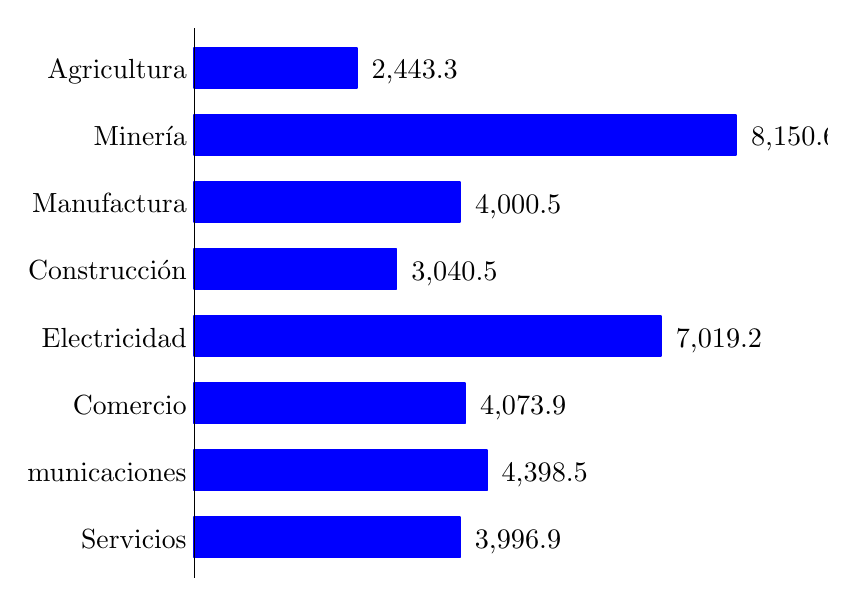
\begin{tikzpicture}[x=1pt,y=1pt]  % Created by tikzDevice version 0.9 on 2016-03-03 04:35:00
% !TEX encoding = UTF-8 Unicode
\definecolor{fillColor}{RGB}{255,255,255}
\path[use as bounding box,fill=fillColor,fill opacity=0.00] (0,0) rectangle (289.08,198.74);
\begin{scope}
\path[clip] (  0.00,  0.00) rectangle (289.08,198.74);

\path[] (  0.00,  0.00) rectangle (289.08,198.74);
\end{scope}
\begin{scope}
\path[clip] (  0.00,  0.00) rectangle (289.08,198.74);

\path[] ( 60.20,  0.00) rectangle (256.03,198.74);

\path[] ( 60.20, 14.54) --
	(256.03, 14.54);

\path[] ( 60.20, 38.78) --
	(256.03, 38.78);

\path[] ( 60.20, 63.02) --
	(256.03, 63.02);

\path[] ( 60.20, 87.25) --
	(256.03, 87.25);

\path[] ( 60.20,111.49) --
	(256.03,111.49);

\path[] ( 60.20,135.73) --
	(256.03,135.73);

\path[] ( 60.20,159.96) --
	(256.03,159.96);

\path[] ( 60.20,184.20) --
	(256.03,184.20);
\definecolor{drawColor}{RGB}{0,0,255}
\definecolor{fillColor}{RGB}{0,0,255}

\path[draw=drawColor,line width= 0.6pt,line join=round,fill=fillColor] ( 60.20,  7.27) rectangle (156.23, 21.81);

\path[draw=drawColor,line width= 0.6pt,line join=round,fill=fillColor] ( 60.20, 31.51) rectangle (165.88, 46.05);

\path[draw=drawColor,line width= 0.6pt,line join=round,fill=fillColor] ( 60.20, 55.74) rectangle (158.08, 70.29);

\path[draw=drawColor,line width= 0.6pt,line join=round,fill=fillColor] ( 60.20, 79.98) rectangle (228.85, 94.52);

\path[draw=drawColor,line width= 0.6pt,line join=round,fill=fillColor] ( 60.20,104.22) rectangle (133.25,118.76);

\path[draw=drawColor,line width= 0.6pt,line join=round,fill=fillColor] ( 60.20,128.46) rectangle (156.32,143.00);

\path[draw=drawColor,line width= 0.6pt,line join=round,fill=fillColor] ( 60.20,152.69) rectangle (256.03,167.23);

\path[draw=drawColor,line width= 0.6pt,line join=round,fill=fillColor] ( 60.20,176.93) rectangle (118.90,191.47);
\definecolor{drawColor}{RGB}{0,0,0}

\path[draw=drawColor,line width= 0.1pt,line join=round] ( 60.20,  0.00) -- ( 60.20,198.74);

\node[text=drawColor,anchor=base west,inner sep=0pt, outer sep=0pt, scale=  1.02] at (161.60, 10.57) {3,996.9};

\node[text=drawColor,anchor=base west,inner sep=0pt, outer sep=0pt, scale=  1.02] at (171.25, 34.81) {4,398.5};

\node[text=drawColor,anchor=base west,inner sep=0pt, outer sep=0pt, scale=  1.02] at (163.45, 59.04) {4,073.9};

\node[text=drawColor,anchor=base west,inner sep=0pt, outer sep=0pt, scale=  1.02] at (234.21, 83.28) {7,019.2};

\node[text=drawColor,anchor=base west,inner sep=0pt, outer sep=0pt, scale=  1.02] at (138.62,107.52) {3,040.5};

\node[text=drawColor,anchor=base west,inner sep=0pt, outer sep=0pt, scale=  1.02] at (161.68,131.76) {4,000.5};

\node[text=drawColor,anchor=base west,inner sep=0pt, outer sep=0pt, scale=  1.02] at (261.40,155.99) {8,150.6};

\node[text=drawColor,anchor=base west,inner sep=0pt, outer sep=0pt, scale=  1.02] at (124.27,180.23) {2,443.3};

\path[] ( 60.20,  0.00) rectangle (256.03,198.74);
\end{scope}
\begin{scope}
\path[clip] (  0.00,  0.00) rectangle (289.08,198.74);

\path[] ( 60.20,  0.00) --
	( 60.20,198.74);
\end{scope}
\begin{scope}
\path[clip] (  0.00,  0.00) rectangle (289.08,198.74);
\definecolor{drawColor}{RGB}{0,0,0}

\node[text=drawColor,anchor=base east,inner sep=0pt, outer sep=0pt, scale=  1.00] at ( 57.45, 10.63) {Servicios};

\node[text=drawColor,anchor=base east,inner sep=0pt, outer sep=0pt, scale=  1.00] at ( 57.45, 34.87) {Comunicaciones};

\node[text=drawColor,anchor=base east,inner sep=0pt, outer sep=0pt, scale=  1.00] at ( 57.45, 59.11) {Comercio};

\node[text=drawColor,anchor=base east,inner sep=0pt, outer sep=0pt, scale=  1.00] at ( 57.45, 83.34) {Electricidad};

\node[text=drawColor,anchor=base east,inner sep=0pt, outer sep=0pt, scale=  1.00] at ( 57.45,107.58) {Construcción};

\node[text=drawColor,anchor=base east,inner sep=0pt, outer sep=0pt, scale=  1.00] at ( 57.45,131.82) {Manufactura};

\node[text=drawColor,anchor=base east,inner sep=0pt, outer sep=0pt, scale=  1.00] at ( 57.45,156.06) {Minería};

\node[text=drawColor,anchor=base east,inner sep=0pt, outer sep=0pt, scale=  1.00] at ( 57.45,180.29) {Agricultura};
\end{scope}
\begin{scope}
\path[clip] (  0.00,  0.00) rectangle (289.08,198.74);

\path[] ( 57.45, 14.54) --
	( 60.20, 14.54);

\path[] ( 57.45, 38.78) --
	( 60.20, 38.78);

\path[] ( 57.45, 63.02) --
	( 60.20, 63.02);

\path[] ( 57.45, 87.25) --
	( 60.20, 87.25);

\path[] ( 57.45,111.49) --
	( 60.20,111.49);

\path[] ( 57.45,135.73) --
	( 60.20,135.73);

\path[] ( 57.45,159.96) --
	( 60.20,159.96);

\path[] ( 57.45,184.20) --
	( 60.20,184.20);
\end{scope}
  \end{tikzpicture}}%
{%
	Instituto Guatemalteco de Seguridad Social} %

  %%%%%%%%%%%%%%%%%%%%%%%%%%%%%%%%%%7%%%%%%%%%%%%%%%%%%%%%%%%
  
  \cajota{%
  	Ingreso de afiliados al IGSS por departamento }%
  {%
  En cuanto al salario promedio mensual de trabajadores afiliados cotizantes al IGSS por departamento, Totonicapán y Guatemala tuvieron los mayores, siendo estos de Q 4,209.7 y Q 4,180.2, respectivamente.
  
  Los departamentos con los menores promedios de ingreso, para los afiliados del IGSS en el 2014, fueron Suchitepéquez con Q 3,039.2 y Escuintla con Q 2,900.8.}%
  {%
  	Promedio del ingreso laboral de trabajadores con seguro social según lugar de residencia
  } %
  {%
  	Por departamento, año 2014, en quetzales} %
  {%
  	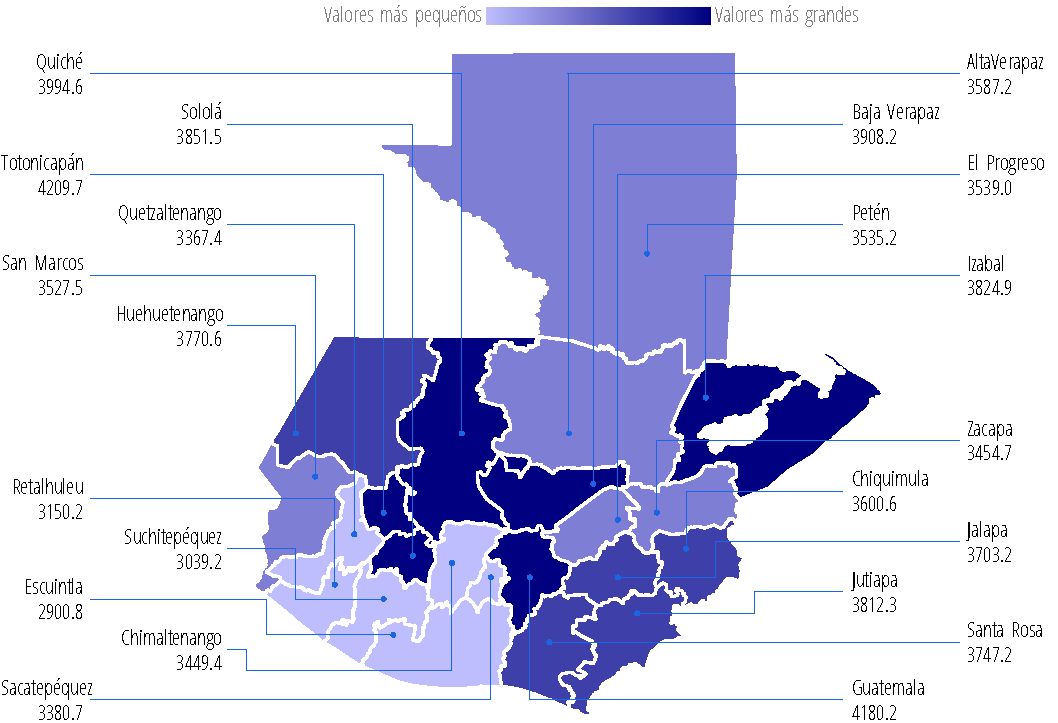
\includegraphics[width=52\cuadri]{graficas/3_06.pdf}}%
  {%
  	Instituto Guatemalteco de Seguridad Social} %

%#########################8########################

\cajita{%
	Costo de la canasta básica}%
{%
En cuanto al acceso de alimentos, en los indicadores sobre el precio de los alimentos, se muestra el costo diario promedio de la canasta básica alimentaria, este fue para el 2015 de Q 113.4.}%
{%
Costo  diario promedio de la canasta básica } %
{%
	República de Guatemala, serie histórica, en quetzales } %
{%
	\begin{tikzpicture}[x=1pt,y=1pt]  % Created by tikzDevice version 0.9 on 2016-03-03 04:35:21
% !TEX encoding = UTF-8 Unicode
\definecolor{fillColor}{RGB}{255,255,255}
\path[use as bounding box,fill=fillColor,fill opacity=0.00] (0,0) rectangle (289.08,198.74);
\begin{scope}
\path[clip] (  0.00,  0.00) rectangle (289.08,198.74);

\path[] (  0.00,  0.00) rectangle (289.08,198.74);
\end{scope}
\begin{scope}
\path[clip] (  0.00,  0.00) rectangle (289.08,198.74);

\path[] (  3.86, 15.61) rectangle (280.54,191.48);

\path[] (  3.86, 18.78) --
	(280.54, 18.78);

\path[] (  3.86, 52.84) --
	(280.54, 52.84);

\path[] (  3.86, 86.90) --
	(280.54, 86.90);

\path[] (  3.86,120.96) --
	(280.54,120.96);

\path[] (  3.86,155.02) --
	(280.54,155.02);

\path[] (  3.86,189.08) --
	(280.54,189.08);

\path[] (  3.86, 35.81) --
	(280.54, 35.81);

\path[] (  3.86, 69.87) --
	(280.54, 69.87);

\path[] (  3.86,103.93) --
	(280.54,103.93);

\path[] (  3.86,137.99) --
	(280.54,137.99);

\path[] (  3.86,172.05) --
	(280.54,172.05);

\path[] ( 35.79, 15.61) --
	( 35.79,191.48);

\path[] ( 88.99, 15.61) --
	( 88.99,191.48);

\path[] (142.20, 15.61) --
	(142.20,191.48);

\path[] (195.41, 15.61) --
	(195.41,191.48);

\path[] (248.62, 15.61) --
	(248.62,191.48);
\definecolor{drawColor}{RGB}{0,0,255}

\path[draw=drawColor,line width= 1.7pt,line join=round] ( 35.79, 60.50) --
	( 88.99, 86.42) --
	(142.20,114.46) --
	(195.41,144.18) --
	(248.62,183.49);
\definecolor{drawColor}{RGB}{0,0,0}

\node[text=drawColor,anchor=base,inner sep=0pt, outer sep=0pt, scale=  1.02] at ( 35.79, 48.59) {77.2};

\node[text=drawColor,anchor=base east,inner sep=0pt, outer sep=0pt, scale=  1.02] at ( 85.87, 86.42) {84.9};

\node[text=drawColor,anchor=base east,inner sep=0pt, outer sep=0pt, scale=  1.02] at (139.07,114.46) {93.1};

\node[text=drawColor,anchor=base east,inner sep=0pt, outer sep=0pt, scale=  1.02] at (191.39,144.18) {101.8};

\node[text=drawColor,anchor=base,inner sep=0pt, outer sep=0pt, scale=  1.02] at (248.62,187.46) {113.4};

\path[draw=drawColor,line width= 0.1pt,line join=round] (  3.86, 23.61) -- (280.54, 23.61);

\path[] (  3.86, 15.61) rectangle (280.54,191.48);
\end{scope}
\begin{scope}
\path[clip] (  0.00,  0.00) rectangle (289.08,198.74);

\path[] (  3.86, 15.61) --
	(  3.86,191.48);
\end{scope}
\begin{scope}
\path[clip] (  0.00,  0.00) rectangle (289.08,198.74);

\path[] (  1.11, 35.81) --
	(  3.86, 35.81);

\path[] (  1.11, 69.87) --
	(  3.86, 69.87);

\path[] (  1.11,103.93) --
	(  3.86,103.93);

\path[] (  1.11,137.99) --
	(  3.86,137.99);

\path[] (  1.11,172.05) --
	(  3.86,172.05);
\end{scope}
\begin{scope}
\path[clip] (  0.00,  0.00) rectangle (289.08,198.74);

\path[] (  3.86, 15.61) --
	(280.54, 15.61);
\end{scope}
\begin{scope}
\path[clip] (  0.00,  0.00) rectangle (289.08,198.74);

\path[] ( 35.79, 12.86) --
	( 35.79, 15.61);

\path[] ( 88.99, 12.86) --
	( 88.99, 15.61);

\path[] (142.20, 12.86) --
	(142.20, 15.61);

\path[] (195.41, 12.86) --
	(195.41, 15.61);

\path[] (248.62, 12.86) --
	(248.62, 15.61);
\end{scope}
\begin{scope}
\path[clip] (  0.00,  0.00) rectangle (289.08,198.74);
\definecolor{drawColor}{RGB}{0,0,0}

\node[text=drawColor,anchor=base,inner sep=0pt, outer sep=0pt, scale=  1.00] at ( 35.79,  2.85) {2011};

\node[text=drawColor,anchor=base,inner sep=0pt, outer sep=0pt, scale=  1.00] at ( 88.99,  2.85) {2012};

\node[text=drawColor,anchor=base,inner sep=0pt, outer sep=0pt, scale=  1.00] at (142.20,  2.85) {2013};

\node[text=drawColor,anchor=base,inner sep=0pt, outer sep=0pt, scale=  1.00] at (195.41,  2.85) {2014};

\node[text=drawColor,anchor=base,inner sep=0pt, outer sep=0pt, scale=  1.00] at (248.62,  2.85) {2015};
\end{scope}
  \end{tikzpicture}}%
{%
	Instituto Nacional de Estadística} %

%#########################9########################

\cajita{%
	Costo de la canasta básica ampliada}%
{%
En cuanto al costo promedio de la canasta básica vital o ampliada, en el 2015 este fue de Q 206.9.

La canasta básica vital incluye gastos de alimentación, vestuario y vivienda.}%
{%
	Costo diario promedio  de la canasta básica ampliada } %
{%
	República de Guatemala, serie histórica, en quetzales } %
{%
	\begin{tikzpicture}[x=1pt,y=1pt]  % Created by tikzDevice version 0.9 on 2016-03-03 04:35:29
% !TEX encoding = UTF-8 Unicode
\definecolor{fillColor}{RGB}{255,255,255}
\path[use as bounding box,fill=fillColor,fill opacity=0.00] (0,0) rectangle (289.08,198.74);
\begin{scope}
\path[clip] (  0.00,  0.00) rectangle (289.08,198.74);

\path[] (  0.00,  0.00) rectangle (289.08,198.74);
\end{scope}
\begin{scope}
\path[clip] (  0.00,  0.00) rectangle (289.08,198.74);

\path[] (  3.86, 15.61) rectangle (280.54,191.48);

\path[] (  3.86, 39.89) --
	(280.54, 39.89);

\path[] (  3.86, 77.26) --
	(280.54, 77.26);

\path[] (  3.86,114.62) --
	(280.54,114.62);

\path[] (  3.86,151.99) --
	(280.54,151.99);

\path[] (  3.86,189.36) --
	(280.54,189.36);

\path[] (  3.86, 21.20) --
	(280.54, 21.20);

\path[] (  3.86, 58.57) --
	(280.54, 58.57);

\path[] (  3.86, 95.94) --
	(280.54, 95.94);

\path[] (  3.86,133.31) --
	(280.54,133.31);

\path[] (  3.86,170.67) --
	(280.54,170.67);

\path[] ( 35.79, 15.61) --
	( 35.79,191.48);

\path[] ( 88.99, 15.61) --
	( 88.99,191.48);

\path[] (142.20, 15.61) --
	(142.20,191.48);

\path[] (195.41, 15.61) --
	(195.41,191.48);

\path[] (248.62, 15.61) --
	(248.62,191.48);
\definecolor{drawColor}{RGB}{0,0,255}

\path[draw=drawColor,line width= 1.7pt,line join=round] ( 35.79, 60.50) --
	( 88.99, 86.30) --
	(142.20,114.41) --
	(195.41,144.13) --
	(248.62,183.49);
\definecolor{drawColor}{RGB}{0,0,0}

\node[text=drawColor,anchor=base,inner sep=0pt, outer sep=0pt, scale=  1.02] at ( 35.79, 48.59) {141.0};

\node[text=drawColor,anchor=base east,inner sep=0pt, outer sep=0pt, scale=  1.02] at ( 84.98, 86.30) {154.8};

\node[text=drawColor,anchor=base east,inner sep=0pt, outer sep=0pt, scale=  1.02] at (138.18,114.41) {169.9};

\node[text=drawColor,anchor=base east,inner sep=0pt, outer sep=0pt, scale=  1.02] at (191.39,144.13) {185.8};

\node[text=drawColor,anchor=base,inner sep=0pt, outer sep=0pt, scale=  1.02] at (248.62,187.46) {206.9};

\path[draw=drawColor,line width= 0.1pt,line join=round] (  3.86, 23.61) -- (280.54, 23.61);

\path[] (  3.86, 15.61) rectangle (280.54,191.48);
\end{scope}
\begin{scope}
\path[clip] (  0.00,  0.00) rectangle (289.08,198.74);

\path[] (  3.86, 15.61) --
	(  3.86,191.48);
\end{scope}
\begin{scope}
\path[clip] (  0.00,  0.00) rectangle (289.08,198.74);

\path[] (  1.11, 21.20) --
	(  3.86, 21.20);

\path[] (  1.11, 58.57) --
	(  3.86, 58.57);

\path[] (  1.11, 95.94) --
	(  3.86, 95.94);

\path[] (  1.11,133.31) --
	(  3.86,133.31);

\path[] (  1.11,170.67) --
	(  3.86,170.67);
\end{scope}
\begin{scope}
\path[clip] (  0.00,  0.00) rectangle (289.08,198.74);

\path[] (  3.86, 15.61) --
	(280.54, 15.61);
\end{scope}
\begin{scope}
\path[clip] (  0.00,  0.00) rectangle (289.08,198.74);

\path[] ( 35.79, 12.86) --
	( 35.79, 15.61);

\path[] ( 88.99, 12.86) --
	( 88.99, 15.61);

\path[] (142.20, 12.86) --
	(142.20, 15.61);

\path[] (195.41, 12.86) --
	(195.41, 15.61);

\path[] (248.62, 12.86) --
	(248.62, 15.61);
\end{scope}
\begin{scope}
\path[clip] (  0.00,  0.00) rectangle (289.08,198.74);
\definecolor{drawColor}{RGB}{0,0,0}

\node[text=drawColor,anchor=base,inner sep=0pt, outer sep=0pt, scale=  1.00] at ( 35.79,  2.85) {2011};

\node[text=drawColor,anchor=base,inner sep=0pt, outer sep=0pt, scale=  1.00] at ( 88.99,  2.85) {2012};

\node[text=drawColor,anchor=base,inner sep=0pt, outer sep=0pt, scale=  1.00] at (142.20,  2.85) {2013};

\node[text=drawColor,anchor=base,inner sep=0pt, outer sep=0pt, scale=  1.00] at (195.41,  2.85) {2014};

\node[text=drawColor,anchor=base,inner sep=0pt, outer sep=0pt, scale=  1.00] at (248.62,  2.85) {2015};
\end{scope}
  \end{tikzpicture}}%
{%
	Instituto Nacional de Estadística} %
